\documentclass[preprint,12pt]{elsarticle}
\usepackage{etoolbox}
\makeatletter
\patchcmd{\ps@pprintTitle}{\footnotesize\itshape
       Preprint submitted to \ifx\@journal\@empty Elsevier
       \else\@journal\fi\hfill\today}{\relax}{}{}
\makeatother

%% Use the option review to obtain double line spacing
%% \documentclass[preprint,review,12pt]{elsarticle}

%% Use the options 1p,twocolumn; 3p; 3p,twocolumn; 5p; or 5p,twocolumn
%% for a journal layout:
%% \documentclass[final,1p,times]{elsarticle}
%% \documentclass[final,1p,times,twocolumn]{elsarticle}
%% \documentclass[final,3p,times]{elsarticle}
%% \documentclass[final,3p,times,twocolumn]{elsarticle}
%% \documentclass[final,5p,times]{elsarticle}
%% \documentclass[final,5p,times,twocolumn]{elsarticle}

%% The graphicx package provides the includegraphics command.
\usepackage{graphicx}
%% The amssymb package provides various useful mathematical symbols
\usepackage{amssymb}
%% The amsthm package provides extended theorem environments
%% \usepackage{amsthm}

%% The lineno packages adds line numbers. Start line numbering with
%% \begin{linenumbers}, end it with \end{linenumbers}. Or switch it on
%% for the whole article with \linenumbers after \end{frontmatter}.
\usepackage{lineno}
\usepackage{url}
\bibliographystyle{unsrt}

%% natbib.sty is loaded by default. However, natbib options can be
%% provided with \biboptions{...} command. Following options are
%% valid:

%%   round  -  round parentheses are used (default)
%%   square -  square brackets are used   [option]
%%   curly  -  curly braces are used      {option}
%%   angle  -  angle brackets are used    <option>
%%   semicolon  -  multiple citations separated by semi-colon
%%   colon  - same as semicolon, an earlier confusion
%%   comma  -  separated by comma
%%   numbers-  selects numerical citations
%%   super  -  numerical citations as superscripts
%%   sort   -  sorts multiple citations according to order in ref. list
%%   sort&compress   -  like sort, but also compresses numerical citations
%%   compress - compresses without sorting
%%
%% \biboptions{comma,round}

% \biboptions{}

\begin{document}

\begin{frontmatter}

%% Title, authors and addresses

\title{Picolo: Fast, Decentralized Globally Distributed Database Network\tnoteref{title1}}
\tnotetext[title1]{Work in progress, Version 0.1 Draft.}

\author{Adi Kancherla, Arunesh Mishra\corref{auth1}}
\cortext[auth1]{Email: adi,arunesh@picolo.network}
\address{San Francisco, California}

%% use the tnoteref command within \title for footnotes;
%% use the tnotetext command for the associated footnote;
%% use the fnref command within \author or \address for footnotes;
%% use the fntext command for the associated footnote;
%% use the corref command within \author for corresponding author footnotes;
%% use the cortext command for the associated footnote;
%% use the ead command for the email address,
%% and the form \ead[url] for the home page:
%%
%% \title{Title\tnoteref{label1}}
%% \tnotetext[label1]{}
%% \author{Name\corref{cor1}\fnref{label2}}
%% \ead{email address}
%% \ead[url]{home page}
%% \fntext[label2]{}
%% \cortext[cor1]{}
%% \address{Address\fnref{label3}}
%% \fntext[label3]{}


%% use optional labels to link authors explicitly to addresses:
%% \author[label1,label2]{<author name>}
%% \address[label1]{<address>}
%% \address[label2]{<address>}

\begin{abstract}
%% Text of abstract
Picolo is a fast, scalable, verifiable, fully-decentralized, globally distributed transaction oriented database for
blockchain-based Applications. Picolo uses a probabilistic replication framework on top of DHTs to achieve a O(1)
lookup latency for most queries. Its the first and so-far only system of its kind to distribute data at a global
scale will full-decentralization and externally-consistent distributed transactions.

\begin{itemize}
    \item Allows for verifiable transaction logs.
    \item Token economics that gamify honest participation from nodes over malicious intent.
\end{itemize}
\end{abstract}

\begin{keyword}
Decentralization \sep Blockchain \sep Crypto economics \sep Database \sep Distributed \sep SQL
%% keywords here, in the form: keyword \sep keyword

%% MSC codes here, in the form: \MSC code \sep code
%% or \MSC[2008] code \sep code (2000 is the default)

\end{keyword}

\end{frontmatter}
%-----------------------------------------------------------------------------
%  INTRODUCTION
%-----------------------------------------------------------------------------
\section{Introduction}\label{Sect:Introduction}


    \begin{itemize}
        \item What are Dapps. Dapps will grow, but need to store data.
        \item Solutions today provide file storage semantics which might not work for all application types.
        \item Introduce the database problem on the blockchain. What are the requirements for a decentralized database.
        \item Overview of current approaches and limitations (details in the Background and Related work section).
    \end{itemize}


\subsection{Picolo's Features}
\begin{itemize}
    \item Network layer Scales with O(log N) overhead for N nodes.
    \item Network lookup using O(1) amortized lookup cost for DHT.
    \item Horizontally scalable 
    \item Automated data sharding
    \item Transactions can be applied across rows, columns and tables across machines
    \item Client controlled replication and data placement
    \item Synchronous replication and external consistency, the strongest form of consistency any database can support
    \item SQL like interface
    \item Supports storage of typed data
    \item Supports semi-relational structure for tables
    \item Configurable backups and restore mechanisms
    \item Verifiable legder for transactions.
\end{itemize}

%-----------------------------------------------------------------------------
%  BACKGROUND SECTION
%-----------------------------------------------------------------------------
\section{Background}
    \begin{itemize}
        \item item
    \end{itemize}

%-----------------------------------------------------------------------------
%  RELATED WORK SECTION
%-----------------------------------------------------------------------------
\section{Overall Design}

    \begin{itemize}
        \item Overall Picolo architecture.
        \item Token economics.
    \end{itemize}
\section{Network Subsystem}

    \begin{itemize}
        \item DHT layer for lookup. Replication and caching for O(1) lookups for popular items.
        \item Token economics for incentivized participation.
        \item Building with BFT. 
    \end{itemize}
\section{Database Subsystem}

\subsection{Cluster}
\subsection{Versioning}
\subsection{Consensus, Replication and Token economics}
\subsection{Handling Failures}
\subsection{Recovery from failures}
\subsection{Clients}
\subsection{Query execution}
\subsection{Sharding}
\subsection{Transactions and hybrid time}

\begin{table}[h]
\centering
\begin{tabular}{l l l}
\hline
\textbf{Treatments} & \textbf{Response 1} & \textbf{Response 2}\\
\hline
Treatment 1 & 0.0003262 & 0.562 \\
Treatment 2 & 0.0015681 & 0.910 \\
Treatment 3 & 0.0009271 & 0.296 \\
\hline
\end{tabular}
\caption{Table caption}
\end{table}


\begin{equation}
\label{eq:emc}
e = mc^2
\end{equation}

Some factors that affect prices of cryptos are listed below. These factors are by no means exhaustive but provide a
framework within which mechanisms to analyze them can be discussed. See the sub sections where some techniques are
presented. \cite{Picolo_Whitepaper}
Factors affecting the prices of crypto assets:

\section{Verifiable data structures, encryption, data sovereignty}

\section{Attacks on the system}


%-----------------------------------------------------------------------------
%  CONCLUSIONS
%-----------------------------------------------------------------------------
\section{Conclusion}
Initial implementations of AI algorithms that analyze structured and unstructured data are discussed. Unstructured data is analyzed in two steps: first, at a unit level and second as a sequence by feeding it to an LSTM. Structured data consisting of live feed from exchanges, current and past bets on the platform amongst others is represented as a game state where an independent decision making agent learns to take actions that maximize its game score. A method of determining payouts to platform users is discussed where they are determined by the magnitude as well as the category of contribution.


%-----------------------------------------------------------------------------
%  BIBLIOGRAPHY
%-----------------------------------------------------------------------------
\section{References}
\bibliography{./bib/picolo.bib}
\end{document}

%% The Appendices part is started with the command \appendix;
%% appendix sections are then done as normal sections
%% \appendix

%% \section{}
%% \label{}

%% References
%%
%% Following citation commands can be used in the body text:
%% Usage of \cite is as follows:
%%   \cite{key}          ==>>  [#]
%%   \cite[chap. 2]{key} ==>>  [#, chap. 2]
%%   \citet{key}         ==>>  Author [#]

%% References with bibTeX database:


%% Authors are advised to submit their bibtex database files. They are
%% requested to list a bibtex style file in the manuscript if they do
%% not want to use model1-num-names.bst.

%% References without bibTeX database:

% \begin{thebibliography}{00}

%% \bibitem must have the following form:
%%   \bibitem{key}...
%%
%% Example figure:
%%
%% \begin{figure}[h]
%% \centering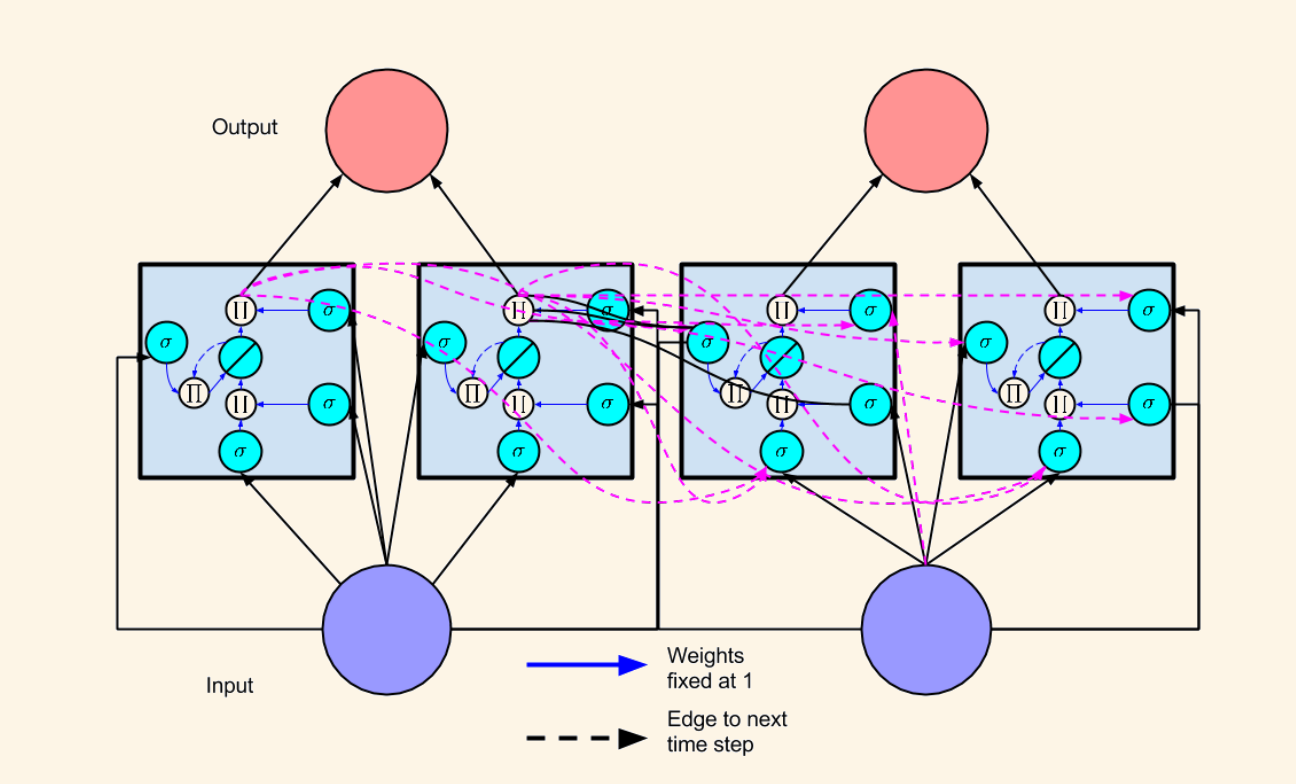
\includegraphics[width=0.4\linewidth]{placeholder.png}
%% \caption{Figure caption}
%% \end{figure}
%% 
% \bibitem{}

% \end{thebibliography}
